\documentclass[letterpaper,11pt]{article}

% Palatino typeface for all text
\usepackage{tgpagella}

% Typesetting mathematics
\usepackage{eulervm}

% Remove hyphenation
\usepackage[none]{hyphenat}
% Maintain justification after removing hyphenation
\sloppy

% Crimson Text and fancy text stuff (like pasting unicode into your .tex file)
% \usepackage{crimson}
\usepackage[T1]{fontenc}
% \usepackage{fontspec}
\usepackage[utf8]{inputenc}
\usepackage[english]{babel}

% Customize page, text, section headings, and quotes
\usepackage[top=1in, bottom=1.5in, left=1.5in, right=1.5in]{geometry}
\usepackage{titlesec}
\usepackage{setspace}
\usepackage[begintext=``,vskip=\partopsep,leftmargin=0.5in,rightmargin=0.5in]{quoting}

% runin: make the abstract heading be part of the paragraph.
\usepackage[runin]{abstract}

% First, make footnotes flush w/ the bottom of the page even if there's some
% remnant whitespace. Second, I like my footnotes to be clickable to get to
% their original location in the text.
\usepackage[bottom]{footmisc}
\usepackage{footnotebackref}

\usepackage{graphicx}
\usepackage{xcolor}

% Caption requirements
\usepackage[
  tableposition=top,
  figureposition=bottom,
  labelfont=bf,
  labelsep=period,
  justification=centering,
]{caption}
\DeclareCaptionFont{8.5pt}{
    \fontsize{8.5pt}{14pt}\selectfont
    \spaceskip=1.0\fontdimen2\font plus 1.0\fontdimen3\font minus 1.0\fontdimen4\font
}
\captionsetup{font=8.5pt}

% Control space around table and figure captions
\captionsetup[figure]{aboveskip=8pt}
\captionsetup[figure]{belowskip=-17pt}
\captionsetup[table]{aboveskip=13pt}
\captionsetup[table]{belowskip=0pt}

% Customize tabular environment as per JDF 2.0
\let\oldtabular\tabular
\let\endoldtabular\endtabular
\renewenvironment{tabular}{
    \fontsize{8.5}{8.5}\selectfont
    \spaceskip=1.0\fontdimen2\font plus 1.0\fontdimen3\font minus 1.0\fontdimen4\font
    \oldtabular}{\endoldtabular}

% Custom space above and below \midrule horizontal line
\usepackage{booktabs}
\aboverulesep=0.5em
\belowrulesep=0.3em

\usepackage{float}      % better figures
\usepackage{enumitem}   % better lists
\usepackage{fancyhdr}   % better headers/footers
\usepackage{hyperref}   % better links

% Make math prettier
\usepackage{amsmath}
\usepackage{amssymb}

% Use APA citation format
\usepackage[natbibapa]{apacite}
\usepackage{natbib}
\setlength\bibhang{0.5in}

% Get the References section to be numbered as if it were created via \section
\usepackage[numbib]{tocbibind}


% Remove the comma between authors and years.
\AtBeginDocument{%
  \renewcommand{\BBAY}{}%% punctuation between authors and year
  % \renewcommand{\BBN}{: }%% punctuation between year and page number
  \renewcommand{\BBYY}{; }%% punctuation between multiple years
}

% Main body spacing
\setstretch{1.26}

% Abstract margins and style
\setlength{\absparindent}{0em}
\setlength{\absleftindent}{0.5in}
\setlength{\absrightindent}{0.5in}
\setlength{\abstitleskip}{-\absparindent}
\renewcommand{\abstracttextfont}{\normalfont}
\abslabeldelim{ \textemdash}
\renewcommand{\abstractnamefont}{\normalfont\bfseries\itshape}

% Paragraph indentation
\setlength{\parindent}{0pt}
\setlength{\parskip}{8.5pt}

% Level 1
\titleformat{\section}
  {\normalfont\fontsize{11}{0}\bfseries}
  {\thesection}{2pt}{\MakeUppercase}

% Level 2
\titleformat{\subsection}
  {\normalfont\fontsize{11}{0}\bfseries}
  {\thesubsection}{2pt}{}

% Level 3
\titleformat{\subsubsection}
  {\normalfont\fontsize{11}{0}\bfseries\itshape}
  {\textup{\thesubsubsection}}{2pt}{}

% Level 4 (The use of headings beyond Heading 3 is discouraged.)
\titleformat{\paragraph}[runin]
  {\normalfont\fontsize{11}{0}\bfseries\itshape}
  {\theparagraph}{2pt}{}

% Level 5 (Not specified in JDF 2.0)
% \titleformat{\subparagraph}
%   {\normalfont\fontsize{11}{0}\itshape}
%   {\theparagraph}{1em}{}

\titlespacing*{\section}{0pt}{7pt}{0pt}
\titlespacing*{\subsection}{0pt}{4.5pt}{0pt}
\titlespacing*{\subsubsection}{0pt}{4.5pt}{0pt}
\titlespacing*{\paragraph}{0pt}{4.5pt}{0pt}

% (Not specified in JDF 2.0)
% \titlespacing*{\subparagraph}{0pt}{8.5pt}{8.5pt}
% \titlespacing*{\subsubparagraph}{0pt}{8.5pt}{8.5pt}

% Just have the page number centered in footer.
\renewcommand{\headrulewidth}{0pt}
\setlength{\footskip}{0.5in}
\fancyhf{}
\cfoot{\thepage}
\pagestyle{fancy}

% Overwrite the title format, specifying font sizes and tightening space between
% the title text and the author.
%
% TODO: Make the spacing between lines a little bigger; things are too tight.
\makeatletter
\renewcommand{\maketitle}{\bgroup
   \begin{center}
   {\fontsize{17pt}{20}\selectfont \@title}
   \vspace{10pt}
   {\fontsize{11pt}{0}\selectfont \@author}
   \vspace{-11pt}
   \end{center}
}
\makeatother

% A pleasant blue to use for links.
\definecolor{ballblue}{HTML}{2ea3f2}

% Set a 0.5in margin for lists.
\setlist{leftmargin=0.5in}
\setlist{nolistsep}

% Increase interword spacing to match with JDF 2.0.
\spaceskip=1.5\fontdimen2\font plus 1.5\fontdimen3\font minus 1.5\fontdimen4\font

% Custom commands: superscript, subscript, and URL.
\newcommand{\super}[1]{$^{\text{#1}}$}
\newcommand{\subsc}[1]{$_{\text{#1}}$}
\newcommand{\link}[2]{\href{#1}{\underline{\smash{#2}}}}

% Custom \authoremail command that adds a clickable email
\newcommand{\authoremail}[2]{\author{#1\\\link{mailto:#2}{#2}}}

% Custom command for inline code-style
\usepackage{courier}
\usepackage{xcolor}
\definecolor{light-gray}{gray}{0.95}
\newcommand{\code}[1]{\colorbox{light-gray}{\texttt{#1}}}

% Sets up some nice PDF metadata
\hypersetup{
  pdftitle={},    % whatever your title is, or some shorter version
  pdfauthor={},   % your name, probably
  pdfsubject={},  % tags or a subject
  % bookmarks=true,
  % bookmarksopen=true,
  pdfpagemode=UseOutlines,
  colorlinks,
  citecolor=ballblue,
  urlcolor=ballblue,
  linkcolor=ballblue
}



\title{
  {{-cookiecutter.project_title_line_1-}} \\

  
    {{-cookiecutter.project_title_line_2-}} \\
  

  
    {{-cookiecutter.project_title_line_3-}} \\
  
  }

\authoremail{ {{-cookiecutter.author_name-}} }{ {{-cookiecutter.author_email-}} }

\begin{document}
\maketitle
\thispagestyle{fancy}

{{cookiecutter.project_description}}

% You may include a new tex file here using:
% \input{<file_name>.tex}

\begin{abstract}
If you are writing a paper that requires an abstract, it should be placed at the
top of the first page underneath the title and author, preceded by the word
Abstract in bold. An extra half-inch should be added to the left and right side
of the abstract. Note that not all papers require abstracts; only those that
would benefit from giving a high-level summary of the project or its background.
\end{abstract}

\section*{Introduction}
Hi! Welcome to Joyner Document Format (JDF). This document format is an attempt
to avoid all the difficulties we encounter when requiring specific word counts.
By standardizing the page count, we hope to incentivize efficiency with both
words and figures. Plus, having a standard format makes every paper feel more
professional. This format is also available as a Word document.

Most conferences take this approach, but we find that most conference formats
are overkill relative to what we really need for our classes. So, we've created
our own format inspired mostly by Lecture Notes in Computer Science. This format
intends to be more usable than the full LNCS, which would be rather onerous to
use several times per semester.


\section*{Grading}
Note that we will not be applying explicit document checks on your formatting.
Your submission will not be automatically rejected for failure to strictly
adhere to this format. Minor issues that no one would notice organically will
not be held against you. More significant issues, like incorrect font sizes,
incorrect margins, or systematic small errors may be subject to penalties.
Alterations that appear to be specifically intended to shorten or extend a
paper's apparent length may be subject to harsher penalties.


\section*{Text}
All text in JDF should be in the Crimson Text font. The Crimson Text font is
available via Google Fonts, or this zip file.

The paper title should be in 18 point bold font, centered at the top of the
first page. The title may be up to three lines. The author's name and email
should be next unless you want or were asked to submit anonymously, in which
case this should be omitted. For typical assignments, the document title may be
as simple as ``Assignment 1''. More specialized assignments may warrant more
unique paper names, like ``A Proposal to Create a New Document Format''.

Body text in JDF should be 12 points, 1.15 spacing. \textbf{Bold},
\emph{italics}, and \underline{underline} may be used as needed. Hyperlinks may
be inserted in the text, as well as superscripts\super{like this},
subscripts\subsc{like this}, and footnotes.\footnote{This is a footnote. The
footnote should be indicated in the text by a number footnote in superscript
format, and the footnote itself should be in 10 point font at the bottom of the
corresponding page.} Body text should be 1.15 spaced, with 6 points of line
spacing after each paragraph. Paragraphs should not be indented.


\subsection*{Heading 1 and Heading 2}
Heading 1 should be bold and in 18 point font. Heading 2 should be bold and in
14 point font. All headings at all levels should have 12pt spacing before the
heading and 6pt spacing after the heading.

\subsubsection*{Heading 3}
Heading 3 should be bold and 12 point font. Like the other headings, it should
be preceded by 12pt spacing and followed by 6pt spacing.

\paragraph*{Heading 4}
Use of headings beyond Heading 3 is not recommended. If need be, though, Heading
4 should be bold, italicized, and 12 point font. Like the other headings, it
should be preceded by 12pt spacing and followed by 6pt spacing.

\subparagraph*{Heading 5}
Use of headings beyond Heading 3 is not recommended. If need be, though, Heading
5 should be italicized and 12 point font. Like the other headings, it should be
preceded by 12pt spacing and followed by 6pt spacing.


\subsection*{Margins}
Margins should be 1.5 inches on all sides. The page number should be included in
the top right corner of the page in the margin.


\section*{Figures \& Tables}
You are encouraged to use figures in your submissions. An example of a figure
inserted into a paper is below, in \autoref{fig::1}.

\begin{figure}[H]
  \centering
  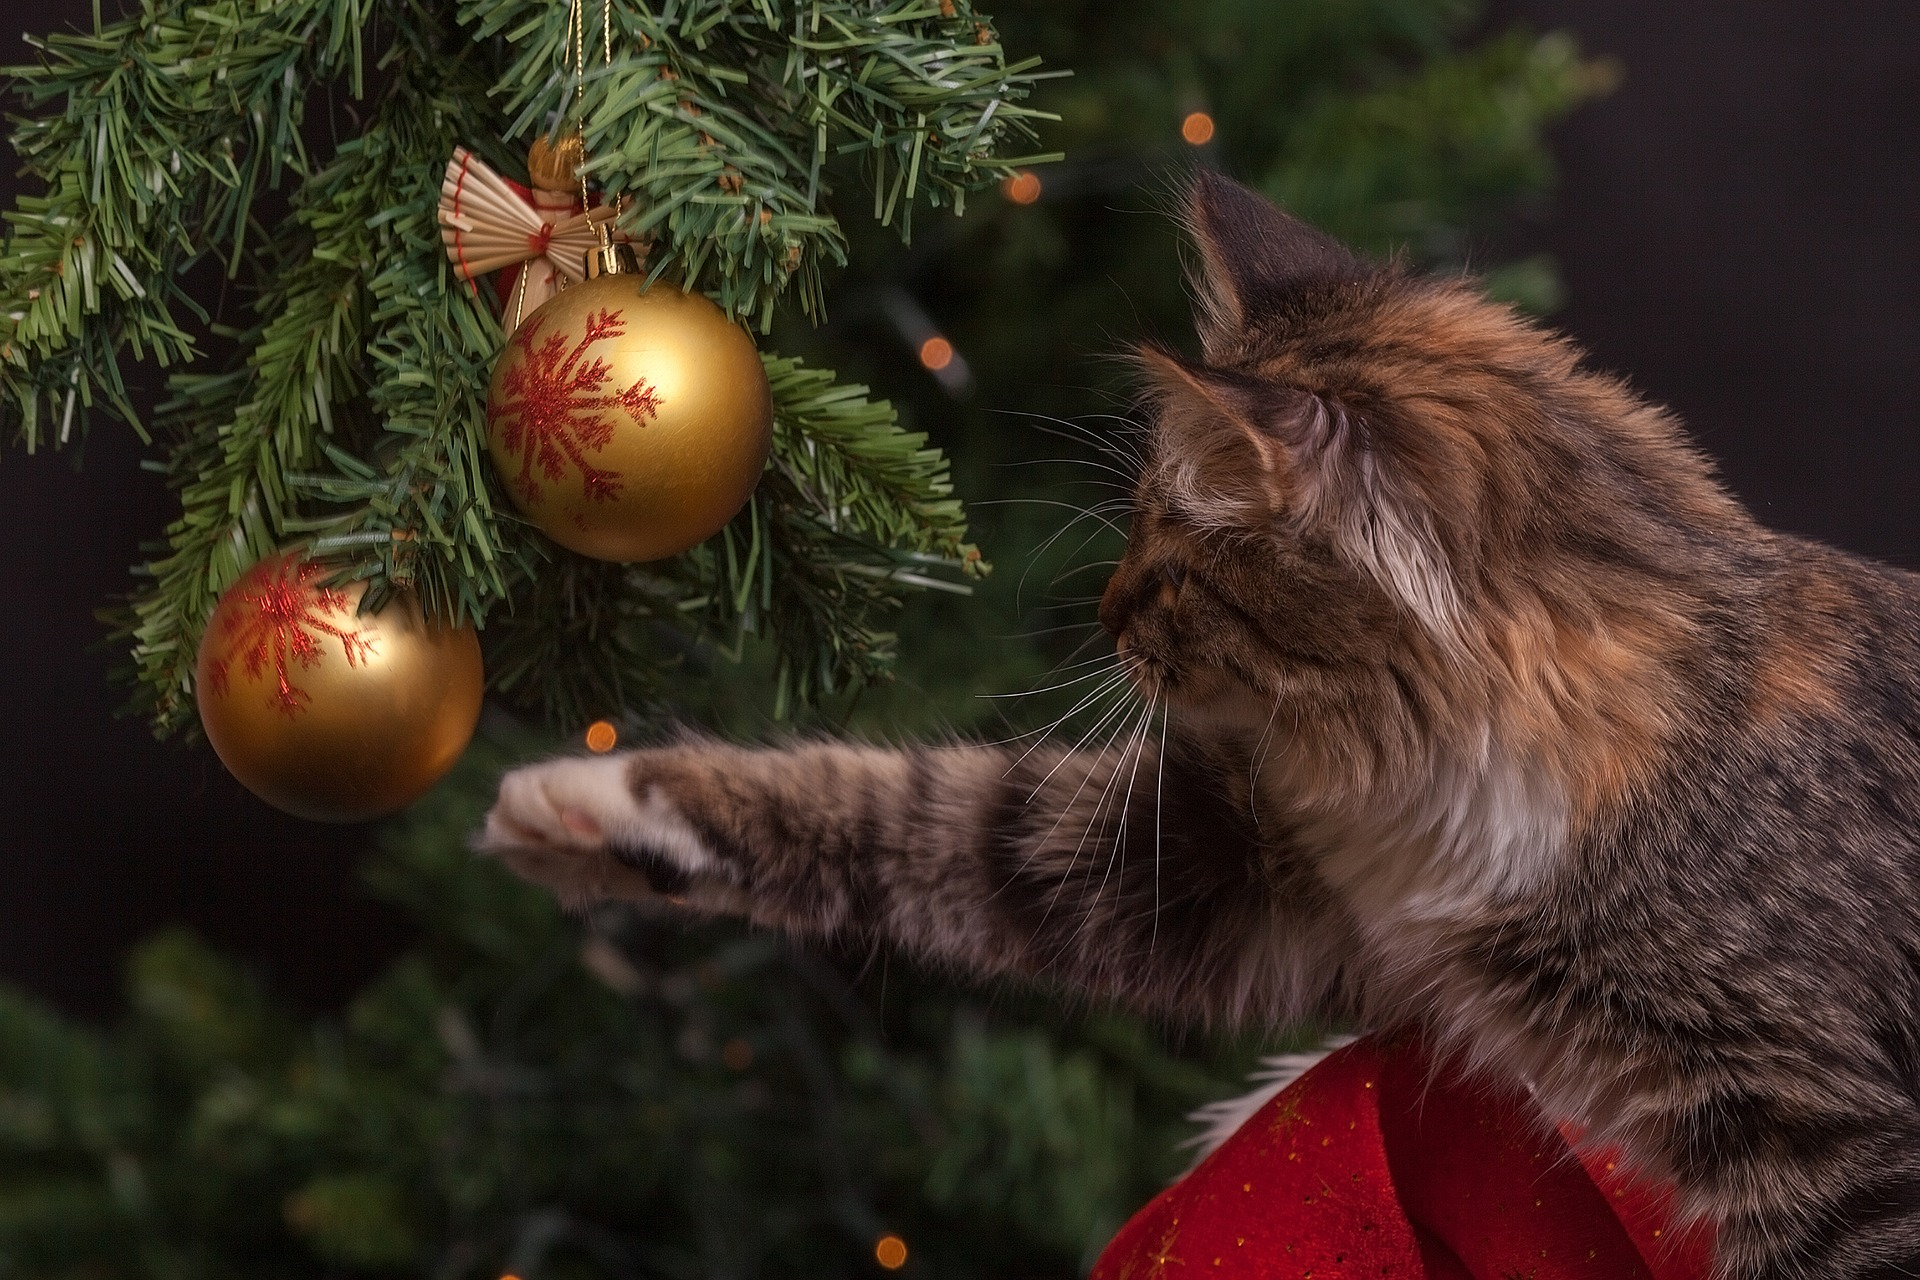
\includegraphics[width=3in, scale=.5]{figs/example-image}
  \caption{The ``New Year's Eve Cat''.}
  \label{fig::1}
\end{figure}

Figures should always be centered on the page, although they may also take up
the entire width of the page. They should not, however, exceed the page margins.
Figures should always be referenced in the text. Figures may also be equations,
diagrams, or other kinds of content.

\subsection*{Figure Captions}
Figures captions should be centered underneath the corresponding figure. The
label for the figure, e.g. ``Figure 1'', should be bolded, and the entire
caption should be 10 point font. If need be, you may have one figure caption
corresponding to multiple consecutive figures, and use either locational
descriptors (e.g. ``Top Left'', ``Middle'') or labels (e.g. ``A'', ``B'') to map
parts of the caption to parts of the figure.

\subsection*{Table Captions}
Table captions should be formatted the same way as figure captions, but they
should be placed above the table. The popular mnemonic for this is:
\underline{f}igures at the \underline{f}oot, \underline{t}ables at the
\underline{t}op. Like figures, tables should not exceed the margins on the page
and should be centered on the page. You have freedom to format the table in the
way that works best for your data.

Make sure that captions are on the same page as the corresponding figure or
table. If a figure or table's size is such that it cannot fit in the text
without leaving considerable blank space on a page or separating the caption
from the table or figure, consider rearranging the text. For example, this
paragraph was moved before the table below so that the table would not span two
pages. You may also place the figure or table and its caption in a textbox with
no outlines and use that to position the figure or table at the top or bottom of
a page while the text rearranges around it.

\begin{table}[H]
  \centering
  \caption{A chart of the number of references to various animals and children in this document.}
  \label{table:1}
  \begin{tabular}{l|c|r}
    \textbf{Value 1} & \textbf{Value 2} & \textbf{Value 3}\\
    $\alpha$ & $\beta$ & $\gamma$ \\
    \hline
    1 & 1110.1 & a\\
    2 & 10.1 & b\\
    3 & 23.113231 & c\\
  \end{tabular}
\end{table}

\section*{Citations and References}
Works should be cited in-line. All works cited in-line should be compiled into a
references list at the end of the paper. APA format is preferred for both
in-line citations and the reference list.

\subsection*{In-line Citations}
Other articles or sources to which you refer should be cited in-line with the
authors' names and the year of publication. The citation should be placed close
in the text to the actual claim, not merely at the end of the paragraph. For
example: students in the OMSCS program are older and more likely to be employed
than students in the on-campus program \citep{Joyner17}. In the event of
multiple authors, list them. For example: research finds sentiment analysis of
the text of OMSCS reviews corresponds to student-assigned ratings of the course
\citep{Newman18}. You may also cite multiple studies together. For example:
several studies have found students in the online version of an undergraduate
CS1 class performed equally with students in a traditional version
\citep{Joyner18a,Joyner18b,Joyner19}. If you would like to refer to an author in
text, you may also do so by including the year (in parentheses) after the
author's name in text. If a publication has more than 4 authors, you may list
only the first author followed by `et al' . For example:
Joyner~et~al.~(\citeyear{Joyner16}) claim that a round of peer review prior to
grading may improve graders' efficiency and the quality of feedback given. This
applies to parenthetical citations as well, e.g. \citep{Joyner16}.

\subsection*{References}
References should be placed at the end of the paper in a dedicated section.
Reference lists should be numbered and organized alphabetically by first
author's last name. If multiple papers have the same author(s) and year, you may
append a letter to the end of the year to allow differentiated in-line text
(e.g. Joyner 2018a and Joyner 2018b in the section above). If multiple papers
have the same author(s), list them in chronological order starting with the
older paper. APA citation and reference style is preferred, but MLA, Chicago,
Harvard, and Vancouver styles are accepted. Only works that are cited in-line
should be included in the references section. For more information on in-line
citations and reference sections, we recommend looking at the
\link{https://owl.purdue.edu/owl/research_and_citation/apa_style/apa_style_introduction.html}{Purdue
Owl}. Note that references are not counted against the length requirements in
any of the listed classes. If the length limit for a particular assignment is 4
pages, then the main text must stop by the end of the fourth page, but the
reference list may extend into and past the 5th page.


\section*{Additional Components}
There are additional components you may need to include in your paper: in-line
quotes, block quotes, bulleted lists, numbered lists, and more.

\subsection*{In-Line and Block Quotes}
If you would like to quote an outside source, you may do so with quotation marks
followed by an in-line citation. If the quote is fewer than three lines, you may
quote it in line. It is acceptable to replace pronouns with their target for
clarity. For example, ``Heavy use of peer grading would compromise [the
school's] reputation'' (Joyner 2016). If a quote is more than three lines, you
should offset it as its own paragraph with half-inch larger margins on each
side. For example:

\begin{quoting}
Whether or not the grades generated by peers are reliably similar to grades
generated by experts is only one factor worth considering, however. Student
perception is also an important factor. A recent study indicated that reliance
on peer grading is one of the top drivers of high MOOC dropout rates. This
problem may be addressed by reintroducing some expert grading where possible''
(Joyner 2016)
\end{quoting}

\subsection*{Bulleted and Numbered Lists}
Bulleted and numbered lists have their text indented a half-inch from the left
margin, with the bullet or number within that space (the standard format for
bullets and margins in Word and Google Docs). For example:
%
\begin{itemize}
\item
  Here's an item.

\item
  Like numbered lists, the second line along a single line in a bulleted list is
  at the same level of indentation.
\end{itemize}

Bulleted lists follow the same format:
%
\begin{enumerate}
\item
  This is an item.
\item
  Note that the left side of the text is aligned, as are the numerals.
\item
  Notice also that a second line corresponding to the same bullet is also
  indented at the same level of the previous lines.
\end{enumerate}

\subsection*{Other Content}
For other content not covered here, you have reasonable flexibility in
determining how it should be used in this format. Generally, nothing should lay
outside the margins. You may specify new types of captions if you would like,
such as Equations, Diagrams, or other kinds of content.


\bibliographystyle{apacite}
\bibliography{references}



\clearpage
\section*{Appendices}
Appendices may be included after the reference list. If you have multiple
appendices, you should label the appendix section in general as a level-1
section called Appendices, and each Appendix with a level-2 header with a label
and title, e.g. ``Appendix A: Interview Transcripts''. If you have only one
appendix, you may simply label it as something like ``Appendix: Interview
Transcript''.

Appendices do not count against the page limit, but appendices should also not
contain any information required to answer the question. The body text should be
sufficient to answer the question, and the appendices should be included only
for you to reference or to give context. Some assignments may also require you
to include certain things in the appendices: these will not count against the
page limit either.

\end{document}
